\section{Polynomial Hierarchy}\label{sec:poly_hierarchy}

\subsection{Hierarchy}\label{subsec:poly_hierarchy}
    The \textit{polynomial hierarchy} is a generalization of \textbf{P}, \textbf{NP} and \textbf{coNP}.

    \begin{definition}[$\Sigma_2^p$]\label{def:sigma_2_p}
        We define the following class for problems with formulas starting with $\exists \forall$ alternation of existentials.

        $ \Sigma_2^p = \{ L \st \exists M,q, x \in L \exists y \in \B^{q(\cardinality{x})} \forall z \in \B^{q(\cardinality{x})} M(x,y,z)=1 \} $
    \end{definition}

    A couple of equivalent definitions of $\Sigma_2^p$:
    \begin{itemize}
        \item $\bm{NP}^{\bm{NP}}$
        \item $ \{ L \st L \preduction \Sigma_2-SAT \} $, where $\Sigma_2-SAT$ is a complete problem for $\Sigma_2^p$ that will be defined later on
    \end{itemize}

    \begin{observation}
        $\Sigma_2^p$ is a superset of the following two classes:
        \begin{itemize}
            \item \textbf{NP} $\subseteq \Sigma_2^p$
            \item \textbf{coNP} $\subseteq \Sigma_2^p$
        \end{itemize}
    \end{observation}

    \begin{definition}[$\Pi_2^p$]\label{def:pi_2_p}
        We define the following class for problems with formulas starting with $\forall \exists$ alternation of existentials.

        $ \Pi_2^p = \{ L \st \exists M,q, x \in L \forall y \in \B^{q(\cardinality{x})} \exists z \in \B^{q(\cardinality{x})} M(x,y,z)=1 \} $
    \end{definition}

    \begin{observation}
        $ L \in \Sigma_2^p \leftrightarrow \bar{L} \in \Pi_2^p $
    \end{observation}

    We can actually generalize these classes in order to account for any number of alternation of quantifiers:
    \begin{itemize}
        \item $\Sigma_i^p$: $\exists \vec{x_1} \forall \vec{x_2} \exists \vec{x_3} \dots Q \vec{x_i} M(x, x_1, x_2, x_3, \dots, x_i) = 1$
        \item $\Pi_i^p$: $\forall \vec{x_1} \exists \vec{x_2} \forall \vec{x_3} \dots Q \vec{x_i} M(x, x_1, x_2, x_3, \dots, x_i) = 1$
    \end{itemize}

    Obviously the last quantifier (i.e. $Q \vec{x_i}$) can be either $\exists$ or $\forall$ depending on the parity of $i$.

    So there comes out the following \textit{polynomial hierarchy} (for better readability, an arrows means $\subseteq$)\footnote{source code of the graph \href{https://en.wikipedia.org/wiki/File:Polynomial_time_hierarchy.svg}{here}}:
    
    \begin{center}
        %\begin{tikzpicture} [   node distance = 1.7cm,
%                        on grid,
%                        state/.style={circle,inner sep=2pt}]
% 
%    % Help grid
%    %\draw [help lines] (-2,2) grid (2,-2);
%     
%    % States
%    \node[black, draw=white] (p)       [state]                     {\textbf{P}};
%    \node[black, draw=white] (np)      [state, above right = of p] {\textbf{NP}$ = \Sigma_1^p$};
%    \node[black, draw=white] (conp)    [state, below right = of p] {\textbf{coNP}$ = \Pi_1^p$};
%    \node[black, draw=white] (sigma2)  [state, right = of np]      {$\Sigma_2^p$};
%    \node[black, draw=white] (pi2)     [state, right = of conp]    {$\Pi_2^p$};
%    \node[black, draw=white] (sigma3)  [state, right = of sigma2]  {$\Sigma_3^p$};
%    \node[black, draw=white] (pi3)     [state, right = of pi2]     {$\Pi_3^p$};
%    \node[black, draw=white] (sigmai)  [state, right = of sigma3]  {$\Sigma_i^p$};
%    \node[black, draw=white] (pii)     [state, right = of pi3]     {$\Pi_i^p$};
%    \node[black, draw=white] (sigmai1) [state, right = of sigmai]  {$\Sigma_{i+1}^p$};
%    \node[black, draw=white] (pii1)    [state, right = of pii]     {$\Pi_{i+1}^p$};
%
%    \path [-stealth, thick]
%        (p) edge [] node {} (np)
%        (p) edge [] node {} (conp)
%        (np) edge [] node {} (sigma2)
%        (np) edge [] node {} (pi2)
%        (conp) edge [] node {} (sigma2)
%        (conp) edge [] node {} (pi2);
%        (sigma2) edge [] node {} (sigma3)
%        (sigma2) edge [] node {} (pi3)
%        (pi2) edge [] node {} (sigma3)
%        (pi2) edge [] node {} (pi3)
%        (sigmai) edge [] node {} (sigmai1)
%        (sigmai) edge [] node {} (pii1)
%        (pii) edge [] node {} (sigmai1)
%        (pii) edge [] node {} (pii1);
        %(sigma2) edge [] node {} (sigma3)
        %(sigma2) edge [] node {} (sigma3)
        %(sigma2) edge [] node {} (sigma3)
        %(sigma2) edge [] node {} (sigma3)
        %(sigma2) edge [] node {} (sigma3)
        %(sigma2) edge [] node {} (sigma3);
     
%\end{tikzpicture}

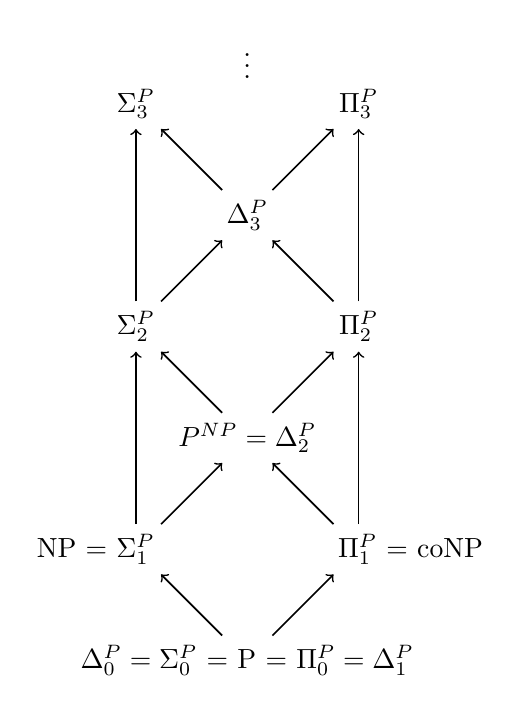
\begin{tikzpicture}[->, node distance=2cm, semithick]
    \node (P) {$\Delta_0^\text{P} =\Sigma_0^\text{P}$ = P = $\Pi_0^\text{P} = \Delta_1^\text{P}$};
    \node (Sigma1) [above left of=P]       {NP = $\Sigma_1^\text{P}$ \hspace*{0.9cm}};
    \node (Pi1)    [above right of=P]      {\hspace*{1.2cm} $\Pi_1^\text{P}$ = coNP};
    \node (Delta2) [above left of=Pi1]     {$\text{P}^\text{NP} = \Delta_2^\text{P}$};
    \node (Sigma2) [above left of=Delta2]  {$\Sigma_2^\text{P}$};
    \node (Pi2)    [above right of=Delta2] {$\Pi_2^\text{P}$};
    \node (Delta3) [above left of=Pi2]     {$\Delta_3^\text{P}$};
    \node (Sigma3) [above left of=Delta3]  {$\Sigma_3^\text{P}$};
    \node (Pi3)    [above right of=Delta3] {$\Pi_3^\text{P}$};
    \node (dots)   [above of=Delta3]       {\vdots};
    \draw (P)      -> (Sigma1);
    \draw (P)      -> (Pi1);
    \draw (Sigma1) -> (Sigma2);
    \draw (Sigma1) -> (Delta2);
    \draw (Pi1)    -> (Pi2);
    \draw (Pi1)    -> (Delta2);
    \draw (Delta2) -> (Sigma2);
    \draw (Delta2) -> (Pi2);
    \draw (Sigma2) -> (Sigma3);
    \draw (Sigma2) -> (Delta3);
    \draw (Pi2)    -> (Pi3);
    \draw (Pi2)    -> (Delta3);
    \draw (Delta3) -> (Sigma3);
    \draw (Delta3) -> (Pi3);
\end{tikzpicture}
        %\fbox{INSERT POLYNOMIAL HIERARCHY DRAWING}
    \end{center}

    It is the number of alternation of quantifiers that is important, not the number of quantifiers itself.

    We know that this hierarchy exists, but we don't know much else; it could even be that everything is equal to \textbf{P}.

    \begin{definition}[\textbf{PH}]\label{def:ph}
        \[ \bm{PH} = \bigcup_i \Sigma_i^p = \bigcup_i \Pi_i^p \]
    \end{definition}

    It is unknown if the hierarchy stops at some point, that is, if $\Sigma_i^p = \Pi_i^p$ for some $i$.
    It that were the case, two things would happen:
    \begin{itemize}
        \item  $\forall j \geq i$ $\Sigma_j^p = \Pi_j^p$
        \item \textbf{PH} = $\Sigma_i^p = \Pi_i^p$
    \end{itemize}

    We say that the hierarchy collapses at the $i$-th level.


\subsection{Complete problems}\label{subsec:ph_complete_problems}
    Let $\Sigma_i-SAT$ be the decision problem asking whether a formula of the form $\exists \vec{x_1} \forall \vec{x_2}, \dots Q \vec{x_i} F(x_1, x_2, \dots, x_i)$ is satisfiable.
    Such problem is complete for $\Sigma_i^p$.

    For $\Pi_i^p$ we have equivalent complete problems, except the alternation of quantifiers is swapped.

    Is there a complete problem for \textbf{PH}?
    Suppose there exists a problem $L$ complete for \textbf{PH}. Surely $L$ is in the hierarchy; i.e. $L \in \bigcup_i \Sigma_i^p$.
    So there is some $i^*$ s.t. $L \in \Sigma_{i^*}^p$.
    Because $L$ is complete for \textbf{PH}, then \textbf{PH} $\preduction \Sigma_{i^*}^p$, which implies that \textbf{PH}$= \Sigma_{i^*}^p$.
    The hierarchy would collap to the $i^*$-th level.


\begin{theorem}[Karp-Lipton]\label{thm:karp_lipton}
    \textbf{NP} $\subseteq$ \textbf{P/poly} $\rightarrow$ \textbf{PH} $= \Sigma_2^p$
\end{theorem}

\begin{theorem}\label{thm:bpp_in_polyhierarchy}
    \textbf{BPP} $\subseteq$ $\Pi_2^p \cap \Sigma_2^p$
\end{theorem}